\section{Results}
\label{sec:results}
% =====================================================================

\subsection{Masked spatial reconstruction across \MSSections{} sections}

\inputtable{tab_multisection}

\begin{figure}[t]
  \centering
  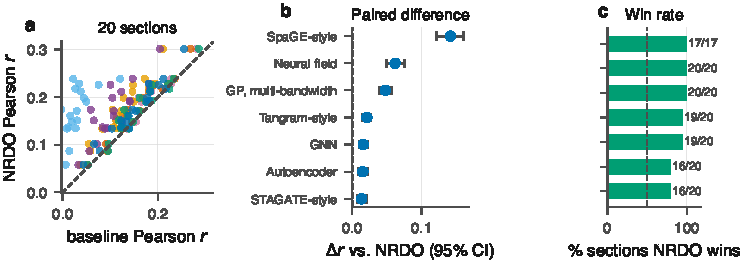
\includegraphics[width=\linewidth]{figures/fig_multisection.pdf}
  \caption{\textbf{Benchmark across \MSSections{} tissue sections.} (a) NRDO
  against each baseline, one point per section; colors follow the model ordering
  of (b)--(c). (b) Mean paired difference with a percentile bootstrap 95\% CI
  over sections. (c) Fraction of sections on which NRDO wins. Every confidence
  interval excludes zero.}
  \label{fig:multisection}
\end{figure}

We evaluate on \MSSections{} sections spanning four technologies
(\MSRuns{} runs), with the section as the unit of analysis: every model sees
identical held-out blocks, so a paired test removes the between-section variance
that otherwise dominates. NRDO attains Pearson $r$ \MSNMOPearson{} against
\MSBestBaselinePearson{} for the closest baseline (\MSBestBaseline{}).

All \MSNBaselines{} baselines are beaten with Holm-corrected
$p \le \MSMaxHolm$ (Appendix~\ref{app:empirical}), and the \emph{smallest} effect size
across the family is $d_z = \MSMinDz$, which is large by conventional
standards; NRDO wins on at least \MSMinWins{} of \MSNPairs{} sections against
every comparator. The advantage is therefore consistent across anatomies rather
than an artifact of one tissue: the twelve MERFISH sections span the
anterior--posterior axis of the same brain with assay, panel and preprocessing
held fixed, so the variation between them is anatomical.

\paragraph{The gain comes from continuity, not from message passing.}
Two controls localize the effect, both measured on this benchmark. A non-spatial
autoencoder sees no coordinates and reaches \MSAEPearson{} purely through the
inverse-distance read-out head shared by every graph baseline, so the gap between
it and a graph model isolates \emph{message passing}: across \MSNGraphModels{}
graph models that margin spans \MSWorstGraphOverAE{} to \MSBestGraphOverAE{}
Pearson $r$, against \MSNMOOverAE{} for NRDO --- an order of magnitude larger. An
implicit neural field (SIREN), which is continuous by construction but carries no
dynamics, is the weakest model tested (\MSWeakestPearson{}, a gap of
$\MSMaxDelta$ against NRDO). Continuity alone is therefore not sufficient, and on
these sections message passing adds little over a well-chosen read-out head; it
is the \emph{operator} that carries the gain, which the parameter-matched $T{=}0$
control confirms directly (Section~\ref{sec:ablations}).

\paragraph{Spatial autocorrelation.}
NRDO leads on SSIM (\MSNMOSSIM{} against \MSBestAnySSIM{} for the best baseline,
\MSBestAnySSIMModel{}) but has by some margin the largest error in Moran's $I$
(\MSNMOMoran{} against \MSBestAnyMoran{} for \MSBestAnyMoranModel{}, a deficit of
\MSMoranDelta{}): the predicted fields are markedly more spatially autocorrelated
than the measurements. On the primary Visium section, where the diagnostic can be
read directly, the predicted map has $I = \NMOMoranPred$ against \MoranTrue{}
measured. SSIM measures local contrast on a rasterized map and Moran's $I$
global autocorrelation on the point set, and the pattern is the expected
signature of a dissipative operator attenuating high spatial frequencies --- the
same diffusion-driven smoothing analyzed for graph neural diffusion
\citep{grand2021,gread2022}. Section~\ref{sec:limitations} discusses the remedy.

\iffullpaper
\subsection{The numerical machinery is load-bearing}
\label{sec:numerics}

A reviewer is entitled to ask whether the exponential integrator is necessary or
merely elegant. Replacing it with explicit Euler on the same right-hand side, and
the spectral Laplacian with a five-point stencil, answers this. The exponential
scheme was stable at every step size tested, up to $\Delta t = \NumStableDt$, or
$\NumCFLRatio\times$ the CFL bound; since it never destabilized, that ratio is a
lower bound imposed by the sweep grid rather than a measured threshold, which is
what Proposition~\ref{prop:contraction} predicts. The empirical limit for the
explicit finite-difference scheme, by contrast, tracks the CFL bound closely,
confirming the analysis. To integrate a fixed horizon to a $10^{-2}$ relative
tolerance the exponential scheme needs \NumStrangSteps{} steps against
\NumEulerSteps{} for explicit Euler, a $\NumSpeedup\times$ difference in cost
(Appendix~\ref{app:empirical}; the step grid is coarse and Euler overshoots the
tolerance, so this is an upper bound on the ratio at that accuracy).
The fair statement is therefore not that the alternatives fail but that they are
an order of magnitude more expensive for the same answer, while additionally
imposing a step-size restriction that couples to \emph{learned} parameters and
can be violated mid-training as $\mD_\theta$ adapts.

\subsection{The reconstruction does not degrade tissue-level structure}
\label{sec:biology}


Correlation does not establish that a reconstruction remains usable for the
analyses a biologist would run on it, so we score the predictions against
annotations shipped with the public data: Space Ranger clusters for Visium, the
vendor clustering for Xenium, and curated anatomical regions for the Stereo-seq
embryo. Clustering the \emph{predicted} expression at held-out locations, NRDO
retains \BioARIRet{} of the adjusted Rand index obtainable from the measured
data, against \BioARIRetBest{} for the best baseline; it is also nominally ahead
on marker AUROC (\BioMarker{} versus \BioMarkerBest{}) and on $k$-NN neighborhood
preservation (\BioKNN{} versus \BioKNNBest{}).

We deliberately do not read these as a second win. Each margin is a small
fraction of its own dispersion --- $\BioARIRetGapSD$, $\BioMarkerGapSD$ and
$\BioKNNGapSD$ pooled standard deviations respectively --- over
\BioSections{} annotated sections, which is too few to support a paired test, and
we report none. The defensible conclusion is the negative one, and it is the one
we intend: the operator attains its reconstruction accuracy \emph{without}
degrading the tissue-level structure a downstream analysis depends on, where a
model that smoothed its way to a good correlation would have lost it. The
reference labels are themselves the output of a clustering algorithm rather than
independent ground truth, which further limits how hard this evidence can be
pushed.

\subsection{Learned dynamics}


\paragraph{The recovered length scale is close to its own initialization.}
On the primary section the fitted operator has a median diffusion length of
\NullBaseline\,$\mu$m. An earlier version of this work noted that this is the
same order as measured morphogen gradients \citep{kicheva2007kinetics,yu2009fgf8}.
That observation does not survive a control, and we report the control instead.

Refitting the identical architecture at the identical budget on
\emph{coordinate-shuffled} sections --- expression permuted across positions, so
every gene's marginal is preserved and no spatial structure remains --- recovers
\NullShuffled\,$\mu$m, against \NullInit\,$\mu$m for the untrained model. The
shuffled fit therefore moves the length scale by \NullShuffledShift\% from
initialization while attaining $r = \NullShuffledR$, and real tissue moves it by
\NullDataShift\%. The initialization is not incidental: it is
$\sqrt{2\,D_{\mathrm{init}}\,\Delta t\,n_{\mathrm{steps}}}$ times the coordinate
scale, fixed by the configuration before any data is seen. Fixing the splat
bandwidth across \NullSigmaRange{} grid cells leaves the result between
\NullSigmaLo{} and \NullSigmaHi\,$\mu$m, and sweeping the lattice over
\NullGridN{} resolutions leaves it between \NullGridUmLo{} and
\NullGridUmHi\,$\mu$m while the same quantity measured in lattice cells moves
from \NullGridCellsLo{} to \NullGridCellsHi. Neither the encoder kernel nor the
discretization is therefore the mechanism: the length is pinned in microns and
free in cells, which is what a quantity fixed in normalized coordinates before
training does (Appendix~\ref{app:empirical}).

We therefore withdraw the correspondence with measured gradient lengths: the
median is largely a configuration constant, and agreement with a biological
scale that a configuration choice also produces is not evidence. What the data
do determine is the \emph{spread}: at initialization every channel carries an
identical length scale, and training differentiates them across
\DiffLenLo--\DiffLenHi\,$\mu$m. The anisotropy is
used rather than merely available: constraining $\mD$ to be isotropic costs
\AblIsotropicDelta{} Pearson $r$.

The dispersion relation (Fig.~\ref{fig:dynamics}c) decreases monotonically in
$|\vk|$, so the fitted operator is dissipative and supports no Turing band. This
is what the training objective selects for: \eqref{eq:steady} rewards making the
\emph{observed} configuration stationary, whereas a Turing-unstable operator
would render the homogeneous state unstable so that structure grows
spontaneously. Recovering a pattern-forming regime would require observations
away from steady state, in line with Theorem~\ref{thm:identifiability}.

\subsection{Transfer across tissue, species and resolution}

Transfer is the weakest setting here, and a protocol caveat governs it. The
zero-shot condition conditions a model on a random half of the target and scores
the complement, whereas every other experiment in this paper scores contiguous
held-out blocks. Those are not equally hard: on the Xenium target the median
distance from a scored location to the nearest visible one is
\SplitXenRandom\,$\mu$m under the random split against \SplitXenBlock\,$\mu$m
under blocks, a factor of \SplitXenRatio{} (Appendix~\ref{app:empirical}). The
random split therefore admits exactly the neighbor leakage that motivated our
block protocol, so zero-shot numbers are comparable to each other but not to the
in-domain oracle or the training-mean floor, and we read only the former.

Under that common protocol, NRDO applied unchanged from adult mouse brain to
human breast carcinoma attains \TissueZeroShot{}, and an operator fitted to
55\,$\mu$m Visium spots and evaluated on single-cell Xenium sampling of the same
organ reaches \ResZeroShot{} over \ResSharedGenes{} shared genes. The
\TissueZeroShotBaselineName{} baseline transfers better in both settings
(\TissueZeroShotBaseline{} cross-tissue) and decoder-only refitting recovers
\TissueFineTune{}. We attribute this to the mechanism that produces the
in-domain gain: NRDO fits an operator whose fixed point is the source tissue, and
relaxation toward that attractor is less appropriate when the target has a
different architecture, whereas local message passing encodes less about the
source. Proposition~\ref{prop:nystrom} makes the distinction precise ---
discretization invariance of the \emph{encoder} does not entail portability of
the \emph{fitted} operator. Conditioning $\mD_\theta$ on tissue-level covariates
is the natural next step. Full tables, the developmental-forecasting result and
the corrected-protocol discussion are in Appendix~\ref{app:empirical}.

\subsection{Counterfactual perturbation}
\label{sec:results4}

We test whether the latent field encodes pathway-specific structure using a
split-half design: we inject the latent direction that maximally raises one
random half of a morphogen pathway, integrate the operator, and assess whether
the \emph{held-out} half responds preferentially against a permutation null over
matched gene sets. Across \BeadNPathways{} pathways the enrichment does not reach
significance (\BeadNSig{} significant; mean held-out rank \BeadMeanRank\% against
a 50\% chance level).

Theorem~\ref{thm:identifiability} predicts this outcome. The perturbation
displaces $\vz$ off the observed manifold $\mathcal{R}=\vz^\star(\Omega)$, and a
single stationary snapshot places no constraint on $f_\theta$ there. The
correlations between latent channels and pathway scores
(Appendix~\ref{app:empirical}) are therefore best read as reflecting coarse
anatomical structure that pathway scores also track, and we do not interpret them
as evidence of a pathway-specific representation. The experiment does establish a
spatial scale: the response decays to half its peak within \BeadWidth\,$\mu$m,
matching the diffusion lengths of $\mD_\theta$. A second pre-specified probe
against Perturb-seq \citep{norman2019perturbseq} was underpowered
($n=\PSNPerturb$) and we report it as inconclusive (Appendix~\ref{app:empirical}).

% =====================================================================
\else
\subsection{Convergence}
\label{sec:convergence}

The benchmark trains every model for a fixed, reduced number of epochs, which
raises a fair objection: if no model has converged, the observed ordering is a
fact about the budget as much as about the models. Section~\ref{sec:limitations}
previously argued that undertraining compresses differences symmetrically, but
that argument does not establish which ordering is the converged one.

We settle it on \ConvSection{}, chosen because it is the section where the
ordering actually changes with budget. Training every model to a shared
early-stopping criterion on the full section with \ConvSeeds{} seeds
(Appendix~\ref{app:empirical}, Table~\ref{tab:converged}), NRDO attains
\ConvNMO{} against \ConvBest{} for the strongest baseline (\ConvBestModel), and
wins on \ConvWins{}/\ConvNPairs{} seeds against every comparator with
$d_z = \ConvMinDz$--$\ConvMaxDz$. At the benchmark's budget the ordering on this
section is reversed. The budget is therefore \emph{conservative} for NRDO here
rather than neutral, and the honest reading of Table~\ref{tab:multisection} is
that it establishes consistency across anatomy at a fixed budget, not that its
margins are the converged margins. With \ConvNPairs{} seeds we report effect
sizes and the win record rather than a significance claim.

Two findings survive convergence and matter more than the ordering. The
non-spatial autoencoder still matches the graph models --- the best of them
leads it by \ConvGraphOverAE{} Pearson $r$ --- so their near-tie is a property of
this task rather than an artifact of undertraining, which strengthens rather
than weakens the reading in Section~\ref{sec:results}. And NRDO retains the
largest error in Moran's $I$ (\ConvNMOMoran{} against \ConvBestMoran{}), so the
over-smoothing is structural and not a symptom of a truncated budget.

The cost is real: NRDO takes \ConvNMOWall\,s against \ConvBaseWallLo--\ConvBaseWallHi\,s
for the baselines on one CPU, a factor of \ConvSlowdown{} against the slowest of
them.

\subsection{Further results}
The exponential integrator costs
$\NumSpeedup\times$ fewer steps than explicit Euler to reach the same
tolerance; the reconstruction does not degrade spatial-domain structure,
marker localization or $k$-NN neighborhoods; zero-shot transfer retains part
of the learned structure but is beaten by the STAGATE-style baseline; and a
counterfactual perturbation probe returns a null result that
Theorem~\ref{thm:identifiability} predicts in advance. All are reported in
full in the archival version.
\fi
